\chapter{Exact Algorithms}

In this chapter we will describe exact algorithms based on the Symmetric version of the Dantzig-Fulkerson-Johnson formulation \cite{DFJ}. The main problem of this model is that the formulation has $O(2^n)$ SECs, so it is impossible to implement all the constraints in the model since it would result in a very high execution time and memory usage even for small graphs.
\\ For this reason, SECs are added only when necessary to the model, in order to discard solutions with cycles. Using this technique, hopefully, only a small fraction of the $O(2^n)$ SECs will be added to the model.
\\ The main algorithms that make use of this technique to solve TSP instances to optimum (of even considerable size) are Loop Methods and CPLEX Callbacks.

\section{Loop Methods}
On this section we will describe two iterative approaches, originally proposed by \cite{bender}, in order to solve the DFJ model without adding an exponential number of Cycle constraints.
\subsection{Simple Loop}
The first approach, that we called Simple Loop, is presented in Algorithm \ref{alg:simpleloop}.
\\ In line 2, we initialize the model with the variables, the degree constraints and the objective function. 
The algorithm then proceeds solving the problem within a while loop (lines 3-4), and at each iteration we check if the optimal solution has more than one component (line 5). If so, we add, for each component, the corresponding subtour eliminator (line 6). \\Instead, if the optimal solution has one component (lines 7-8), that is, it is a Hamiltonian cycle, then we return the optimal solution found (line 9).
\\ This algorithm turns out very efficient, especially with recent solvers. Its efficiency is due to the fact that the solution is solved very fast, especially in first iterations, and only small number of SECs are added at each iteration. These constraints allow to exclude a lot of solutions with subtours of the original problem. 
\\ At worst, since the problem is NP-hard, all constraints will be added to the model, requiring exponential computational time, but in most cases this doesn't happen.
It may seem that this method is not very efficient, but with recent and increasingly sophisticated solvers, it can lead to the optimal solution, even with many nodes, in few seconds.
\begin{algorithm}
    \caption{Simple Loop}\label{Loop Method}
    \hspace*{\algorithmicindent} \textbf{Input:} $G = (V,E) , \; c : E \rightarrow \mathbb{R}^+$\\
    \hspace*{\algorithmicindent} \textbf{Output:} $\textbf{\textit{z}\text{*}} $ optimal solution to TSP on the input graph $G$
    \begin{algorithmic}[1]
    \State $\textit{done} \gets \textit{false}$
    \State model $ \leftarrow $ \textbf{$\ast$ Initialize variables and objective function $\ast$ }
    \While {!done} 
    	\State $\textbf{\textit{z}\text{*}} \gets \text{optimal\_solution}(\text{model})$\;
	\If{$components(z\text{*}) > 1$} 
	\State \textbf{ $\ast$ Add SECs for each connected component to the model $\ast$ }
	
	\Else \State $\textit{done} \gets \textit{true}$
	\EndIf	
    \EndWhile
    \State \textbf{return} $\textbf{\textit{z}\text{*}} $
    \end{algorithmic}
    \label{alg:simpleloop}
    \end{algorithm}
\noindent
\subsection{Heuristic Loop}
The Algorithm \ref{alg:simpleloop} has a drawback since at each iteration we solve to optimum the TSP problem, even if the constraints collected until that point are not sufficient to achieve the true optimum. In other words, we must wait that the solver finds out the optimal solution, even if the constraints available may allow solutions with subtours.
\\ For this reason, we implemented an ``heuristic" version of the method seen before. This method is composed of two phases. The first phase is used to collect some SECs by relaxing the optimality concept, for example by setting an higher value for the solution GAP or limiting the solution in the root node of the branching tree.
This phase permits to add useful constraints to the model, without computing the optimal solution in each iteration. In fact, with this phase we can obtain a lot of useful SECs in a short time, especially in the first iterations.
This phase remains active until the solution found has more than one component, from then on, it will be activated the second phase. 
In the second phase, the solver's concept of ``relaxation" is removed and it essentially solve the problem with the Simple Loop method, ensuring that the solution returned is the true optimal solution.
\\ The Heuristic Loop is presented in Algorithm \ref{alg:heuloop}. In line 4, as in the first method, we initialize the model with the variables, the degree constraints and the objective function.
At the beginning, the first phase is active (line 2), which means that some CPLEX parameters have to be set (line 5) in order to obtain a non-optimal solution, thus speeding up the computational time. In our case, we decided to set three CPLEX parameters, that is, the MIP gap tolerance, the MIP node limit and the MIP solution limit. The first parameter force CPLEX to stop, when the solution found until that point has a GAP of a certain value (for example 5\%). The second parameter specifies the node of the branching tree until which CPLEX can compute the solution, for example, if the value of the parameter is set to 0, CPLEX can compute the solution only in the root node. The third parameter specifies the maximum number of integer solutions that the solver can compute. \\
The algorithm then proceeds solving the problem within a while loop (line 6). As in the Simple Loop, at each iteration we check if the solution has more than one component, and if so, we add, for each component, the corresponding SEC. \\ Instead, if the optimal solution has one component, we set the flag \textit{second\_phase} to true (line 15) and reset the solver settings, thus ensuring that the solution found from now on it will be an optimal solution.
During the first phase, we have hopefully collected a number of useful SECs in a small amount of time, compared to finding the optimal solution at each iteration.
For the description of the second phase please refer to the Simple Loop (Algorithm \ref{alg:simpleloop}).
\begin{algorithm}
    \caption{Heuristic Loop}\label{Loop Method}
    \hspace*{\algorithmicindent} \textbf{Input:} $G = (V,E) , \; c : E \rightarrow \mathbb{R}^+$\\
    \hspace*{\algorithmicindent} \textbf{Output:} $\textbf{\textit{z}\text{*}} $ optimal solution to TSP on the input graph $G$
    \begin{algorithmic}[1]
    \State $\textit{done} \gets \textit{false}$
    \State $\textit{first\_phase} \gets \textit{true}$
    \State $\textit{second\_phase} \gets \textit{false}$
    \State model $ \leftarrow $ \textbf{$\ast$ Initialize variables and objective function $\ast$ }
    \State CPXsetintparam $ \leftarrow $ \textbf{$\ast$ Set MIP gap tolerance, MIP node limit and MIP solution limit in order to obtain a non-optimal solution $\ast$ }
    \While {!done} 
    	\If{$second\_phase$} 
	\State CPXsetintparam $ \leftarrow $\textbf{ $\ast$ Return to original solver settings in order to obtain an optimal solution $\ast$ }
	\State $\textit{second\_phase} \gets \textit{false}$
	\EndIf
    	\State $\textbf{\textit{z}\text{*}}  \gets \text{optimal\_solution}(\text{model})$\;
	\If{$components(z\text{*}) > 1$} 
	\State \textbf{ $\ast$ Add SECs for each connected component to the model $\ast$ }
	\EndIf
	\If{$ components(z\text{*}) == 1 \And first\_phase$} 
	\State $\textit{first\_phase} \gets \textit{false}$
	\State $\textit{second\_phase} \gets \textit{true}$
	\EndIf
	\If{$ components(z\text{*}) == 1 \And !first\_phase$} 
	\State $\textit{done} \gets \textit{true}$
	\EndIf
    \EndWhile
    \State \textbf{return} $\textbf{\textit{z}\text{*}} $
    \end{algorithmic}
    \label{alg:heuloop}
    \end{algorithm}
    
\newpage
\subsection{Final comparison between Loop Methods}
\label{LMcomparision}
The dataset used to compare exact algorithms consists of 30 instances with four different random seeds \{201909284, 19, 190696, 19061996\}, for a total of 120 runs per algorithm. The instances used are the following:
 \begin{multicols}{3}
    \begin{itemize}
        \item a280.tsp
        \item att48.tsp
        \item att532.tsp
        \item berlin52.tsp
        \item bier127.tsp
        \item ch130.tsp
        \item ch150.tsp
        \item d198.tsp
        \item gil262.tsp
        \item kroA100.tsp
        \item kroA150.tsp
        \item kroA200.tsp
        \item kroB100.tsp 
        \item kroB150.tsp
        \item kroB200.tsp
        \item kroC100.tsp
        \item kroD100.tsp
        \item kroE100.tsp 
        \item lin105.tsp
        \item lin318.tsp 
        \item pr226.tsp 
        \item rat195.tsp 
        \item pr76.tsp 
        \item pr107.tsp 
        \item pr124.tsp
        \item pr136.tsp
        \item tsp225.tsp
        \item u159.tsp
        \item rat99.tsp
        \item rd400.tsp
    \end{itemize}
    \end{multicols}
\noindent
For each problem, we compare the elapsed time to compute the optimal solution.\\
In Figure \ref{fig:loops} it is possible to see the performance profile of the Loop Methods analyzed in this section.
The parameter we used are the following:
\begin{itemize}
 	\item \textbf{Simple Loop:} no parameters;
	\item \textbf{Heuristic Loop:} 
	\begin{itemize} 
		\item \textbf{MIP gap tolerance:} Absolute tolerance on the gap between the best integer objective and the objective of the best node remaining. Value used: 0.05;
		\item \textbf{MIP node limit:} Maximum number of nodes solved before the algorithm terminates. Value used: 0 (only the root node);
		\item \textbf{MIP solution limit:} Number of MIP solutions to be found before stopping. Value used: 1.
		\end{itemize}
\end{itemize}
The parameters for the Heuristic Loop are used in the first phase of the algorithm, then they are reset to their original values to find the optimal solution.
From the graphs we can see that the performance of the two algorithms are very similar. In the first phase of the Heuristic Loop, the SECs found are probably not sufficient to save time during the second phase of the algorithm. In our opinion, there is no reason to use the Heuristic Loop since, even with three parameters, there is always the risk to overtune the parameters using only few instances.

\begin{figure}[h!]
  \centering
  \begin{subfigure}[b]{0.97\linewidth}
    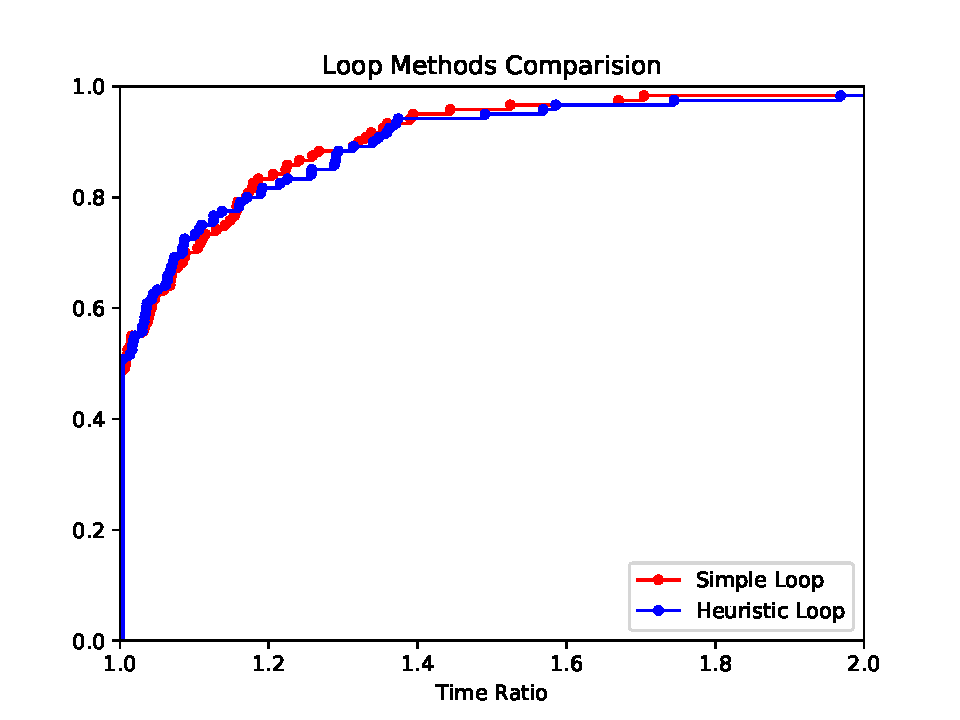
\includegraphics[width=\linewidth]{media/LoopMethods1.pdf}
  \end{subfigure}
  \begin{subfigure}[b]{0.97\linewidth}
    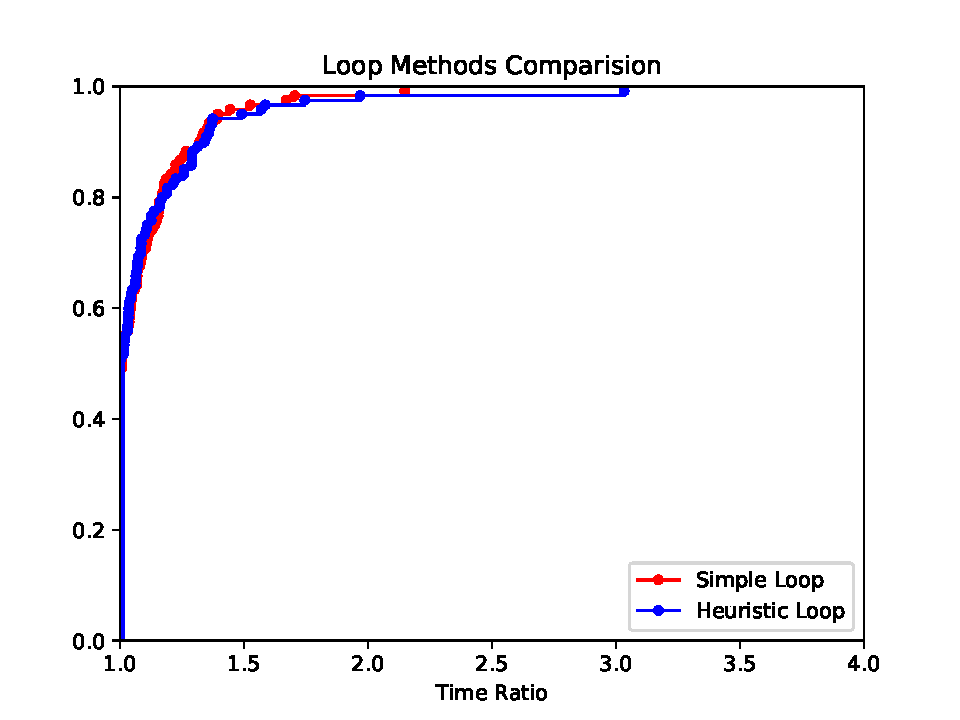
\includegraphics[width=\linewidth]{media/LoopMethods.pdf}
  \end{subfigure}
  \caption{On top: detailed view of the performance profile of Loop Methods. \\On the bottom: full view of the performance profile of Loop Methods.}
  \label{fig:loops}
\end{figure}

\clearpage
\section{Callbacks}
In this section we will describe how to solve the DFJ model using CPLEX callbacks. Until now, the algorithms we described resolve TSP instances with an iterative approach, that is, they solve multiple times a ``relaxed" model, adding the SECs when the solution found is composed of multiple tours. Since CPLEX uses the branch-and-cut technique to solve the MIP model, with the previous approach multiple decision trees will be created from scratch, losing much of the information from previous trees. Another way to handle the SECs is to exploit the branch-and-cut technique. In particular, when an integer solution is found by the solver during the decision tree, we can reject it if contains multiple tours by adding a SEC for each of them. With this method we develop only a single decision tree, and this results, hopefully, in a faster computation. To reach this goal, CPLEX provides a series of callbacks that can be used for adding constraints and solutions on the fly.

\subsection{Lazy Callback}
The lazy callback allows to resolve the TSP in a very fast and natural way. As described previously, in order to solve the problem we must reject solutions that have multiple tours, adding SECs on the fly. This leads to Algorithm \ref{alg:lazycall} in which we instantiate the model and the objective function as usual (line 2). Then we instantiate a procedure called LazyCallback (line 3). A LazyCallback is a function called by the solver when an integer solution is found during the branch-and-cut algorithm. The task of the callback is to check if the solution found has more than one connected component (line 8) and if it is the case, to reject the solution by adding the SECs to the model (lines 9 - 10). After this, the resolution of the model resumes (line 11).
The routine continues by optimally solving the model and returning the solution found (lines 4 - 5).


\begin{algorithm}
    \caption{Lazy Callback}\label{Lazy Callback}
    \hspace*{\algorithmicindent} \textbf{Output:} $\textbf{\textit{z}\text{*}} $ optimal solution to TSP on the input graph $G$
    \begin{algorithmic}[1]
   \Function{TSPopt}{$G = (V,E) , \; c : E \rightarrow \mathbb{R}^+$}
  \State model $ \leftarrow $ \textbf{$\ast$ Initialize variables and objective function $\ast$ }
  \State optimizer $ \leftarrow $ \textbf{$\ast$ Initialize the LazyCallback function within the optimizer $\ast$ }
  \State $\textbf{\textit{z}\text{*}} \gets \text{optimizer(model)}$
  \State \Return \textbf{\textit{z}\text{*}}
\EndFunction
\\
  \Function{LazyCallback}{\textbf{\textit{x}}, model}
  \State comp $ \leftarrow $ \textbf{$\ast$ number of components in the integer solution \textit{x} $\ast$ }
  \If{$ (comp > 1) $} 
	\State \textbf{ $\ast$ Add SECs for each connected component to the model $\ast$ }
	\EndIf  
	\State \Return 
	\EndFunction

    \end{algorithmic}
     \label{alg:lazycall}
    \end{algorithm}

\subsection{UserCut Callback}
Another interesting callback is the UserCut which is used to generate SECs constraints on fractional solutions. The idea is pretty the same as the Lazy callback; when a fractional solution is found during the exploration of the decision tree by the solver, the UserCutCallback function checks the solution and adds constraints to the model on the fly. The procedure is described in algorithm \ref{alg:usercutcall}. In this case both LazyCallback and UserCutCallback must be defined (line 3). In particular, the UserCutCallback function checks how many components there are in the solution (line 14), if there are many connected components then it adds the SECs for each connected component (lines 15 - 16). Instead, when the graph is connected, we apply to the model the violated cuts, looking for sections with a capacity less than a certain threshold. The cutoff value is set to 2.0 - $\epsilon$, with $\epsilon$ = 0.1 in our implementation (lines 17 - 18). We used the \textit{Concorde}\footnote{\url{http://www.math.uwaterloo.ca/tsp/concorde.html}} algorithms in order to fast computing the connected components and violated cuts in fractional solutions. Due to the fact that fractional solutions are more than integer solutions and that the UserCutCallback function employs several time consuming algorithms, the callback is called only when the depth of the decision tree is less than or equal to 10, which is a reasonable tradeoff between number of constraints applied to the model and time spent in executing flow algorithms.



\begin{algorithm}
    \caption{UserCut Callback}\label{UserCut Callback}
    \hspace*{\algorithmicindent} \textbf{Output:} $\textbf{\textit{z}\text{*}} $ optimal solution to TSP on the input graph $G$
    \begin{algorithmic}[1]
   \Function{TSPopt}{$G = (V,E) , \; c : E \rightarrow \mathbb{R}^+$}
  \State model $ \leftarrow $ \textbf{$\ast$ Initialize variables and objective function $\ast$ }
  \State optimizer $ \leftarrow $ \textbf{$\ast$ Initialize the callback functions within the solver $\ast$ }
  \State $\textbf{\textit{z}\text{*}} \gets \text{optimizer(model)}$
  \State \Return \textbf{\textit{z}\text{*}}
\EndFunction
\\
  \Function{LazyCallback}{\textbf{\textit{x}}, model}
  \State comp $ \leftarrow $ \textbf{$\ast$ number of components in the integer solution \textit{x} $\ast$ }
  \If{$ (comp > 1) $} 
	\State \textbf{$\ast$ Add SECs for each connected component to the model $\ast$ }
	\EndIf  
	\State \Return 
	\EndFunction
	\\
	\Function{UserCutCallback}{\textbf{\textit{x}}, model}
  \State comp $ \leftarrow $ \textbf{$\ast$ number of components in the fractional solution \textit{x} $\ast$ }
  \If{$ (comp > 1) $} 
	\State \textbf{$\ast$ Add SECs for each connected component to the model $\ast$ }
	\EndIf
	\If{$ (comp = 1) $} 
	\State \textbf{$\ast$ Add SECs on the separated fractionary solution $\ast$ }
	\EndIf 
	\State \Return 
	\EndFunction

    \end{algorithmic}
    \label{alg:usercutcall}
    \end{algorithm}
    
\subsection{Heuristic Callback}
\label{callHeu}
The last callback that we present is the Heuristic which is used to provide to the solver heuristic feasible solutions from fractional or infeasible solutions. 
In our case, since we are trying to solve the TSP problem, we generate first a tour from integer solutions with multiple connected components and then we add them to the solver using the CPLEX heuristic callback, which permits to add solutions and to automatically check their feasibility. This technique is very useful in the early stages of the branch-and-cut algorithm because, by providing a TSP solution to the solver, we can provide an upper-bound to the optimal solution, in order to cut many branches of the decision tree. This led us to define the Algorithm \ref{alg:heucall}. The main differences with respect to Algorithm \ref{alg:usercutcall} are the addition of a new function called HeuristicCallback and a new algorithm to compute a tour starting from an integer solution with multiple components provided in the LazyCallback function. Since we want the algorithm to be thread safe, we must keep track of the index of each thread that produce a specific solution. To do this, for every integer solution with multiple connected components provided by the Lazy callback, we compute a new solution composed by a single tour (i.e. a TSP solution), saving in addition the index of the thread that has computed that solution (lines 11 - 12).
The algorithm to compute a tour starting from an infeasible solution is presented in Algorithm \ref{alg:completetouralg}. The idea is very simple, combine connected components in a single tour optimizing the total length by merging the most nearest components.
In particular, the algorithm starts by computing the number of components of the solution (line 2). This value correspond to the iterations that the algorithm must perform in order to merge all the components of the solution (line 3). Inside the while loop, the algorithm compute the minimum delta for each pair of nodes of the graph that are in different components. The delta correspond to the incremental cost of the objective function due to a specific swap of edges. Two cases are possible (lines 6 - 13); in the first case, the edge composed of $(a, a^{\prime} = \textit{succ}(a))$ is replaced by $(a, b)$ and the edge $(b, b^{\prime})$ is replaced by $(b^{\prime}, a^{\prime})$, increasing the objective function of $\Delta(a,b)$. In this case, the order of the edges in the second component must be reversed to preserve the correct direction of the graph (Figure \ref{fig:completetour} a - b). The second case is simpler and it is obtained by crossing the edges as in Figure \ref{fig:completetour} c and d. Once the minimum delta is found, the correct swap is applied to the graph (lines 14 - 20) and the number of components is reduced by 1 (line 21 - 22). 
Concluding the description of algorithm 5, when the HeuristicCallback function is called by the solver, it checks whether a solution has been saved for the current thread (line 24) and, if a solution exists, it adds it to the solver, leaving the latter to verify its feasibility (line 25).

\begin{algorithm}
    \caption{Heuristic Callback}\label{Heuristic Callback}
    \hspace*{\algorithmicindent} \textbf{Output:} $\textbf{\textit{z}\text{*}} $ optimal solution to TSP on the input graph $G$
    \begin{algorithmic}[1]
   \Function{TSPopt}{$G = (V,E) , \; c : E \rightarrow \mathbb{R}^+$}
  \State model $ \leftarrow $ \textbf{$\ast$ Initialize variables and objective function $\ast$ }
  
  \State optimizer $ \leftarrow $ \textbf{$\ast$ Initialize the callback functions within the solver $\ast$ }
  \algstore{myalg}
    	\end{algorithmic}
	\label{alg:heucall}
   	\end{algorithm}
	\vspace{1cm}
	\begin{algorithm}                     
   	 \begin{algorithmic} [1]              
    	\algrestore{myalg}
  \State $\textbf{\textit{z}\text{*}} \gets \text{optimizer(model)}$
  \State \Return \textbf{\textit{z}\text{*}}
\EndFunction
\\
  \Function{LazyCallback}{\textbf{\textit{x}}, model}
  \State comp $ \leftarrow $ \textbf{$\ast$ number of components in the integer solution \textit{x} $\ast$ }
  \If{$ (comp > 1) $} 
	\State \textbf{$\ast$ Add SECs for each connected component to the model $\ast$ }
	\State \textbf{\textit{x}$^{\prime}$} $ \leftarrow $ \text{complete\_tour(\textbf{\textit{x}})}
	\State \textbf{$\ast$ Save \textbf{\textit{x}$^{\prime}$} and the thread index $\ast$ }
	\EndIf  
	\State \Return 
	\EndFunction
	\\
	\Function{UserCutCallback}{\textbf{\textit{x}}, model}
  \State comp $ \leftarrow $ \textbf{$\ast$ number of components in the fractional solution \textit{x} $\ast$ }
  \If{$ (comp > 1) $} 
	\State \textbf{$\ast$ Add SECs for each connected component to the model $\ast$ }
	\EndIf
	\If{$ (comp = 1) $} 
	\State \textbf{$\ast$ Add SECs on the separated fractionary solution $\ast$ }
	\EndIf 
	\State \Return 
	\EndFunction
	\\
	\Function{HeuristicCallback}{\textbf{\textit{x}}, model}
	\State \textbf{if} $\ast$ there is a solution available in the current thread $\ast$ \textbf{then}
	\State \textbf{$\ast$ Add the TSP heuristic solution \textbf{\textit{x}$^{\prime}$} to the solver $\ast$ }
	\State \Return 
	\EndFunction

    \end{algorithmic}
    
    \end{algorithm}
    
    \noindent
    
    \begin{algorithm}[H]
    \caption{complete tour}\label{complete tour}
    \hspace*{\algorithmicindent} \textbf{Input:} \textbf{\textit{x}} solution with multiple connected components \\ 
    \hspace*{\algorithmicindent} \textbf{Output:} \textbf{\textit{x}$^{\prime}$} heuristic TSP solution
    \begin{algorithmic}[1]
    \State \textit{min} $\gets \infty$
    \State \textit{ncomp} $\gets $ components(\textbf{\textit{x}})
    
	
    \While {(ncomp != 1)} 
    \ForEach {$a,b \in \mathcal V $}
    \If{$ (comp(a)$  !=  $comp(b)) $} 
	\State $\Delta(a,b) = dist(a, b^{\prime}) + dist(b, a^{\prime}) - dist(a, a^{\prime}) - dist(b, b^{\prime})$
	\If{$ (\Delta(a,b) < min) $} 
	\State $ min = \Delta(a,b) $
	\State \textit{flag} $\gets 0$
	\EndIf 
	\State $\Delta(a,b)^{\prime} = dist(a, b) + dist(b^{\prime}, a^{\prime}) - dist(a, a^{\prime}) - dist(b, b^{\prime})$
	\If{$ (\Delta(a,b)^{\prime} < min) $} 
	\State $ min = \Delta(a,b)^{\prime} $
	\State \textit{flag} $\gets 1$
	\EndIf 
	\EndIf 
    \EndFor
    \algstore{myalg1}
    	\end{algorithmic}
	\label{alg:completetouralg}
   	\end{algorithm}
	\noindent
	\begin{algorithm}                   
   	 \begin{algorithmic} [1]              
    	\algrestore{myalg1}
    \If{$ (flag = 1) $} 
    \State \textbf{$\ast$ reverse the order of edges of the second component $\ast$ }
    \State $ (a, b) \gets (a, a^{\prime})$
    \State $ (b^{\prime}, a^{\prime}) \gets (b, b^{\prime})$
    \EndIf 
    \If{$ (flag = 0) $} 
    \State $ (a, b^{\prime}) \gets (a, a^{\prime})$
    \State $ (b, a^{\prime}) \gets (b, b^{\prime})$
    \EndIf 
    \State \textbf{$\ast$ update components of \textbf{\textit{x}} $\ast$ }
    \State \text{ncomp} $\gets \text{ncomp $-$ 1} $    
    \EndWhile
    \State \textbf{return} $ \textbf{\textit{x}} $
    \end{algorithmic}
    \end{algorithm}

\begin{figure}[h!]
  \centering
  \begin{subfigure}[b]{0.49\linewidth}
    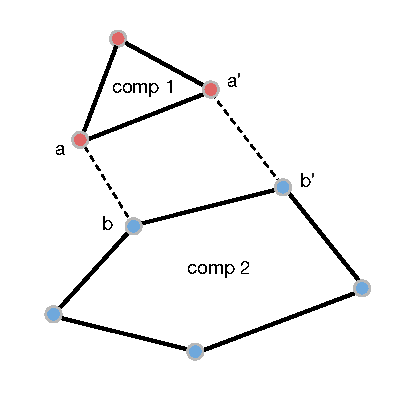
\includegraphics[width=\linewidth]{media/HEU-1__.pdf}
     \caption{First case: before merging}
  \end{subfigure}
  \begin{subfigure}[b]{0.49\linewidth}
    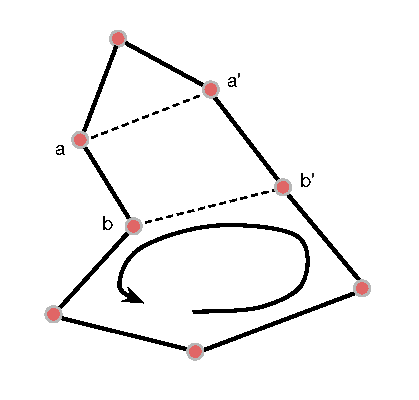
\includegraphics[width=\linewidth]{media/HEU-solved2prova.pdf}
    \caption{First case: after merging}
  \end{subfigure}
  \begin{subfigure}[b]{0.49\linewidth}
    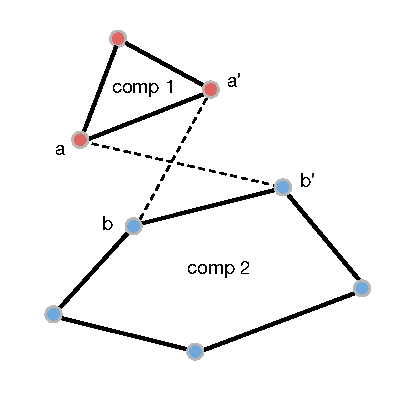
\includegraphics[width=\linewidth]{media/HEU-2_.pdf}
    \caption{Second case: before merging}
  \end{subfigure}
  \begin{subfigure}[b]{0.49\linewidth}
    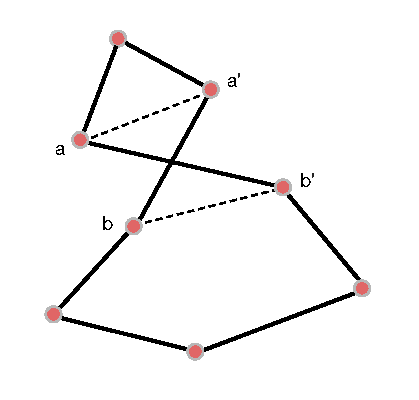
\includegraphics[width=\linewidth]{media/HEU-2solved2prova.pdf}
    \caption{Second case: after merging}
  \end{subfigure}
  \caption{The two ways to merge connected components used by the complete\_tour algorithm.}
  \label{fig:completetour}
\end{figure}
\clearpage
\noindent
Since the overall algorithm is $O(n^2)$, the Heuristic Callback is called only when the depth of the decision tree is less than or equal to 10.
\subsection{Generic Callback}
The Generic Callback is a relatively new function that contains essentially two new features with respect to previous callbacks.
The first one is that the callback, during a call to a user-defined function, doesn't stop the execution of the \textit{Dynamic Search} algorithm. The latter is a branch-and-cut based algorithm, which is kept secret by CPLEX and which guarantee better performance than the traditional but robust branch-and-cut algorithm.
The second feature is that with a single callback we can define each previous callback using the \textit{context}. The context is a CPLEX structure that defines in which part of the brach-and-cut algorithm the solver calls the callback.
An example of the use of Generic Callback is presented in Algorithm \ref{alg:genlazycall}.  This algorithm includes the three callbacks implemented in Algorithm \ref{alg:heucall}, namely, Lazy callback, UserCut Callback and Heuristic Callback. 
The solver calls the generic callback function with the context CANDIDATE when an integer solution is found (line 8). In this case, we simply collected all function included in the Lazy callback and in the Heuristic callback (lines 9 - 15). On the other hand, after each fractional solution found by the solver the context used is RELAXATION (line 16). In this part of the algorithm, we collected all the function included in the UserCut callback together with the Concorde algorithms (lines 17 - 21).

\begin{algorithm}
    \caption{Generic Callback}\label{Generic Callback}
    \hspace*{\algorithmicindent} \textbf{Output:} $\textbf{\textit{z}\text{*}} $ optimal solution to TSP on the input graph $G$
    \begin{algorithmic}[1]
   \Function{TSPopt}{$G = (V,E) , \; c : E \rightarrow \mathbb{R}^+$}
  \State model $ \leftarrow $ \textbf{$\ast$ Initialize variables and objective function $\ast$ }
  \State optimizer $ \leftarrow $ \textbf{$\ast$ Initialize the callback function within the solver $\ast$ }
  \State $\textbf{\textit{z}\text{*}} \gets \text{optimizer(model)}$
  \State \Return \textbf{\textit{z}\text{*}}
\EndFunction
\\
  \Function{GenericCallback}{\textbf{\textit{x}}, context, model}
 
  \If{$ (context = CANDIDATE) $} 
   	\State comp $ \leftarrow $ \textbf{$\ast$ number of components in the integer solution \textit{x} $\ast$ }
	 \If{$ (comp > 1) $} 
	\State \textbf{$\ast$ Add SECs for each connected component to the model $\ast$ }
	\State \textbf{\textit{x}$^{\prime}$} $ \leftarrow $ \text{complete\_tour(\textbf{\textit{x}})}
	\State \textbf{$\ast$ Save \textbf{\textit{x}$^{\prime}$} and the thread index $\ast$ }
	\EndIf  
	\State \textbf{if} $\ast$ there is a solution available in the current thread $\ast$ \textbf{then}
	\State \textbf{$\ast$ Add the TSP heuristic solution \textbf{\textit{x}$^{\prime}$} to the solver $\ast$ }
	\EndIf  
	\If{$ (context = RELAXATION) $} 
   	\State comp $ \leftarrow $ \textbf{$\ast$ number of components in the fractional solution \textit{x} $\ast$ }
	 \If{$ (comp > 1) $} 
	\State \textbf{$\ast$ Add SECs for each connected component to the model $\ast$ }
	\EndIf
		    \algstore{myalg2}
    	\end{algorithmic}
	\label{alg:genlazycall}
   	\end{algorithm}
	\vspace{1cm}
	\begin{algorithm}                   
   	 \begin{algorithmic} [1]              
    	\algrestore{myalg2}
	\If{$ (comp = 1) $} 
	\State \textbf{$\ast$ Add SECs on the separated fractionary solution $\ast$ }
	\EndIf 
	\EndIf  
	\State \Return 
	\EndFunction

    \end{algorithmic}
    \end{algorithm}

\subsection{Final comparison between callbacks}
\label{callbackresults}
For the final comparison of the callbacks we used the same dataset described in Section \ref{LMcomparision}, i.e. 30 instances with four random seeds, for a total of 120 problems.
For the comparison we used two metrics: time elapsed and nodes solved. The first metric is used to compare the time spent by the algorithms to compute the optimal solution of each problem. The second metric is used to compare the number of nodes solved by the algorithms when running the branch-and-cut algorithm. The number of nodes solved can make us understand if the cuts applied by the callbacks are sufficient to prevent the expansion of numerous nodes of the branched tree during the branch-and-cut algorithm. \\
On Figure \ref{fig:lazy} it is possible to see the performance profile of the Legacy Callbacks. In CPLEX the legacy callbacks are the previous version of the new generic callback and \textit{Lazy Callback}, \textit{UserCut Callback} and \textit{Heuristic Callback} are part of this category. The first thing we can notice is that \textit{Lazy Callback} is the one that performs worst. The \textit{Heuristic Callback} seems to be performing slightly better than the \textit{UserCut Callback}. The heuristic solutions provided to the solver using the Heuristic Callback together with the cuts computed in fractional solutions using Concorde, can significantly reduce the amount of time to compute the optimal solution for the TSP problem. The number of nodes solved by the three algorithms is also consistent with the times, as you can see in Figure \ref{fig:lazynodes}. This confirms that cuts and heuristic solutions are capable of cutting many branches of the decision tree. \\
On Figure \ref{fig:gen} it is possible to see the performance profile of the Generic Callbacks. Also in this case the \textit{Heuristic Callback} outperforms all the other both in terms of time and number of solved nodes, as you can see in Figure \ref{fig:gennodes}. \\
In Figure \ref{fig:allcall} we can see the comparison between all the Callbacks. The \textit{Legacy Heuristic Callback} outperforms the others in most of the instances, however it does not do so consistently. In a small percentage of instances it takes a really long time to finish and is outperformed by the \textit{Generic Heuristic Callback}. This means that if we were to look at the percentage of instances solved quickly, the \textit{Legacy Heuristic Callback} is the best method, but the method capable of solving the most of instances within 4 times the time it takes the fastest method to find the optimum is the \textit{Generic Heuristic Callback}. This is followed by the \textit{Generic UserCut Callback} with slightly worse performance and the \textit{Legacy UserCut Callback}.\\ \textit{Lazy Callbacks} are the ones that perform worst. The number of nodes solved by each algorithm is shown in Figure \ref{fig:allcallnodes}. \\
On Figure \ref{fig:exact} it is possible to see the performance profile of the Exact Algorithms. The only new thing to note is that \textit{Loop Methods} perform better than \textit{Legacy Lazy Callback}.
All performance profiles are shown on the following pages.

\begin{figure}[h!]
  \centering
  \begin{subfigure}[b]{0.97\linewidth}
    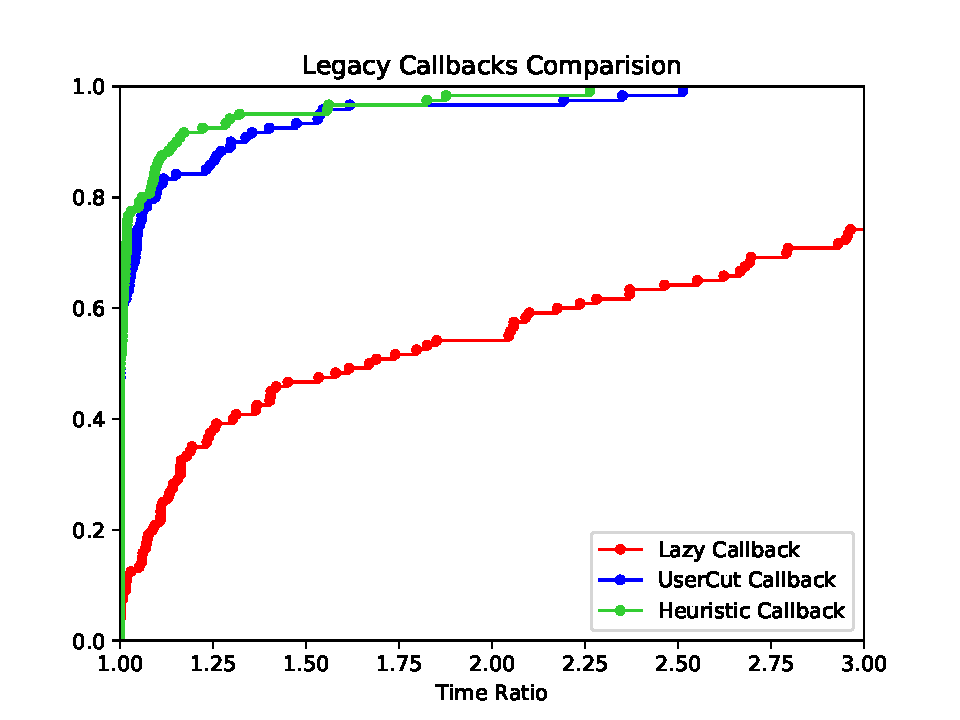
\includegraphics[width=\linewidth]{media/LegacyCallbacks.pdf}
  \end{subfigure}
  \begin{subfigure}[b]{0.97\linewidth}
  \ContinuedFloat
    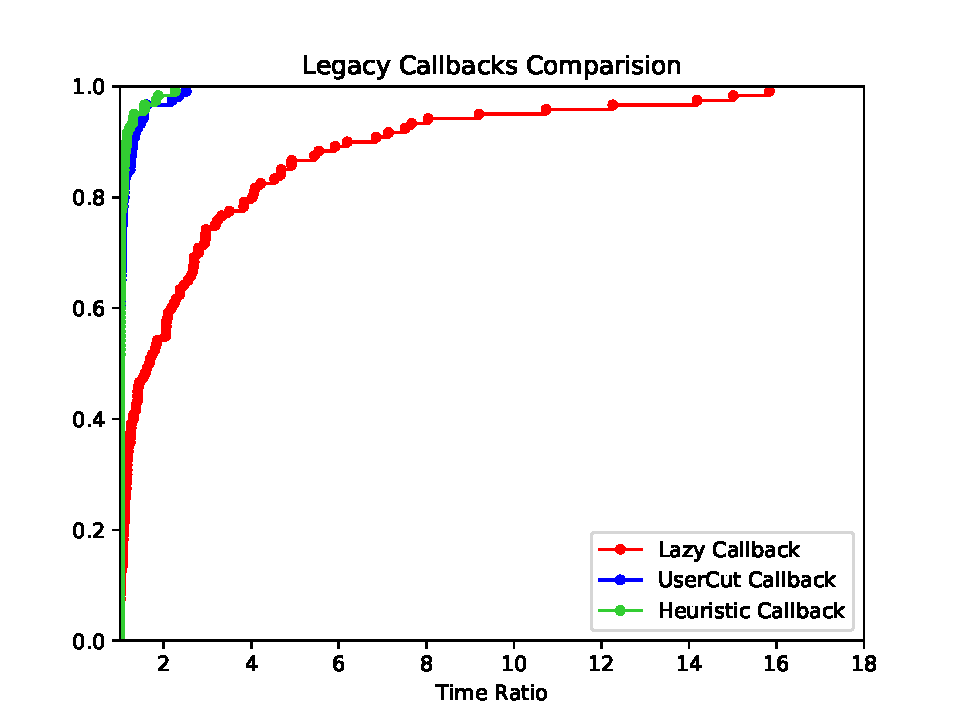
\includegraphics[width=\linewidth]{media/LegacyCallbacks1.pdf}
  \end{subfigure}
  \caption{On top: detailed view of the performance profile of Legacy Callbacks. \\On the bottom: full view of the performance profile of Legacy Callbacks.}
\label{fig:lazy}
\end{figure}

\begin{figure}[h!]
  \centering
  \begin{subfigure}[b]{0.97\linewidth}
    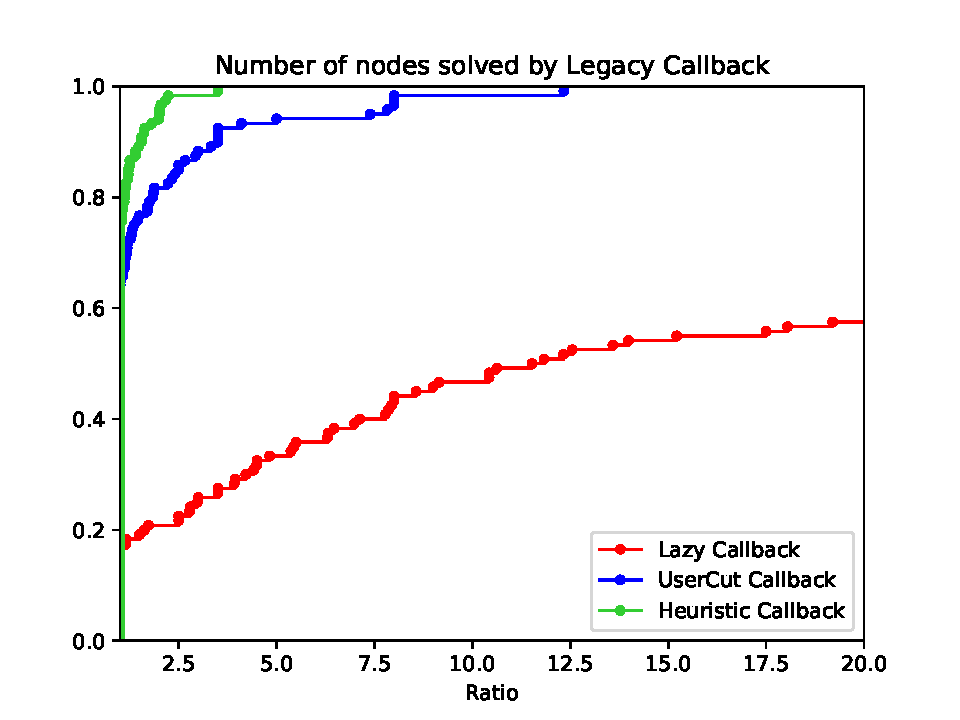
\includegraphics[width=\linewidth]{media/NodesLegacy.pdf}
  \end{subfigure}
  \begin{subfigure}[b]{0.97\linewidth}
  \ContinuedFloat
    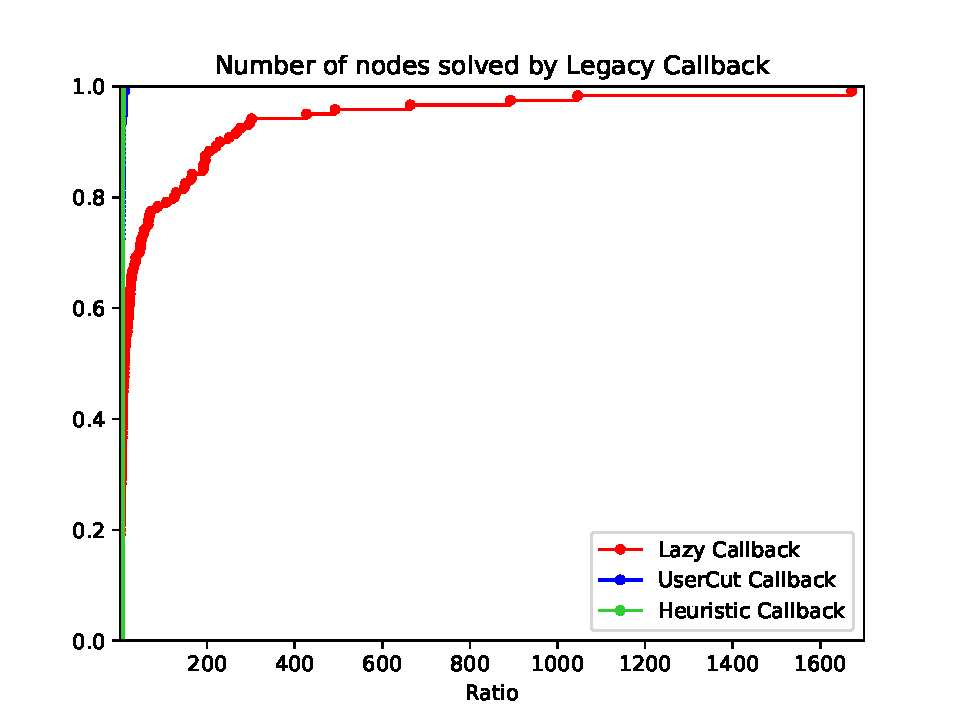
\includegraphics[width=\linewidth]{media/NodesLegacy1.pdf}
  \end{subfigure}
  \caption{On top: detailed view of the performance profile of Legacy Callbacks regarding the number of solved nodes. On the bottom: full view of the performance profile of Legacy Callbacks.}
  \label{fig:lazynodes}
\end{figure}

\begin{figure}[h!]
  \centering
  \begin{subfigure}[b]{0.97\linewidth}
    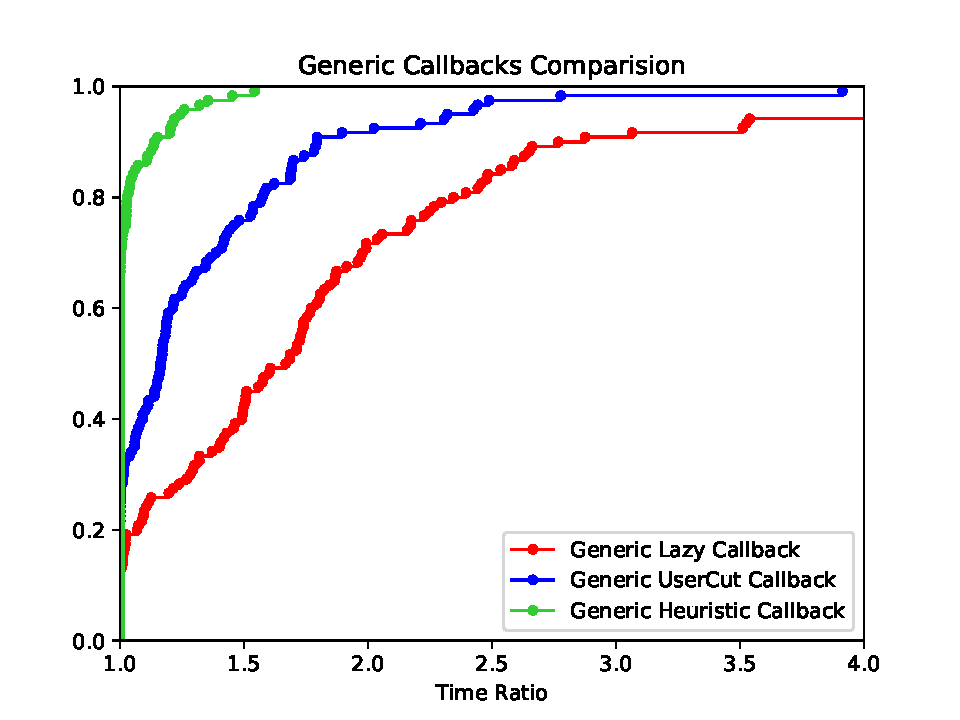
\includegraphics[width=\linewidth]{media/GenericCallbacks.pdf}
  \end{subfigure}
  \begin{subfigure}[b]{0.97\linewidth}
  \ContinuedFloat
    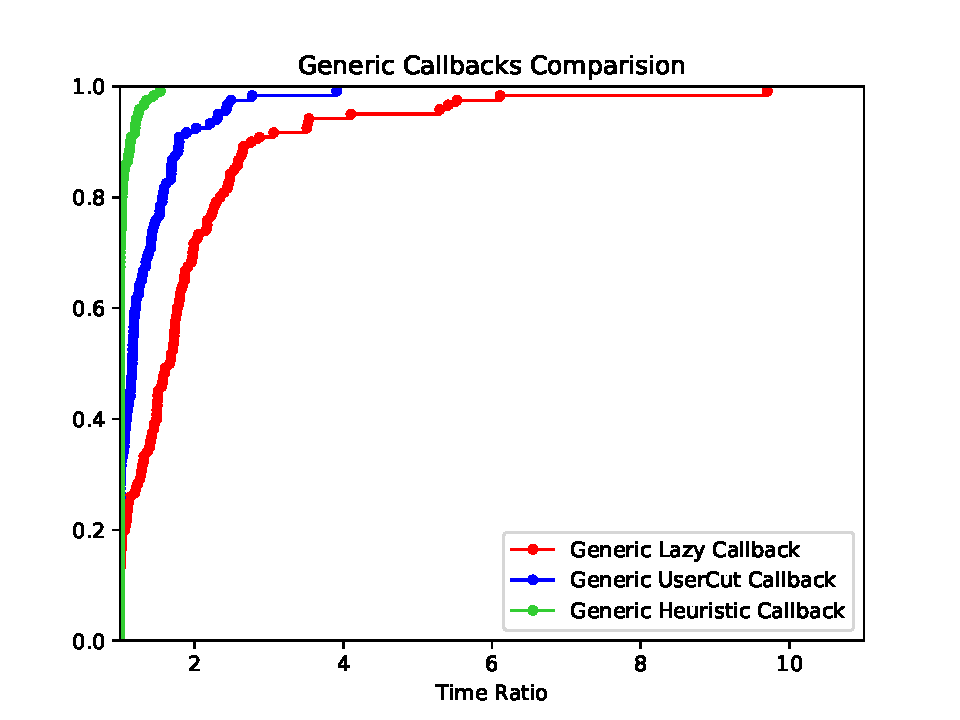
\includegraphics[width=\linewidth]{media/GenericCallbacks1.pdf}
  \end{subfigure}
  \caption{On top: detailed view of the performance profile of Generic Callbacks. \\On the bottom: full view of the performance profile of Generic Callbacks.}
  \label{fig:gen}
\end{figure}

\begin{figure}[h!]
  \centering
  \begin{subfigure}[b]{0.97\linewidth}
    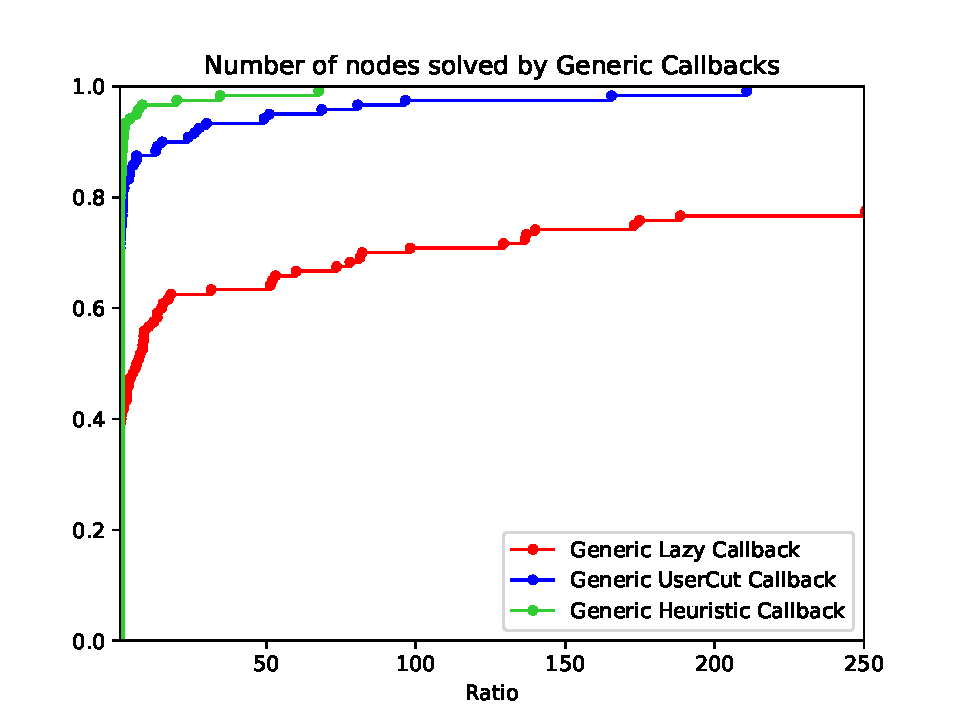
\includegraphics[width=\linewidth]{media/NodesGeneric.pdf}
  \end{subfigure}
  \begin{subfigure}[b]{0.97\linewidth}
  \ContinuedFloat
    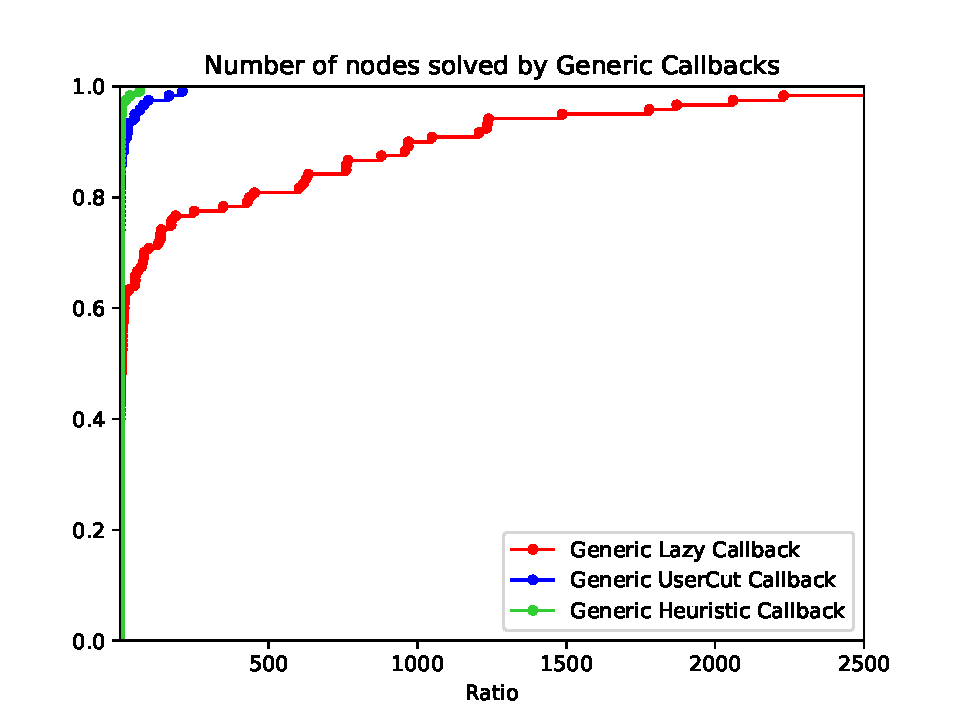
\includegraphics[width=\linewidth]{media/NodesGeneric1.pdf}
  \end{subfigure}
  \caption{On top: detailed view of the performance profile of Generic Callbacks regarding the number of solved nodes. On the bottom: full view of the performance profile of Generic Callbacks.}
    \label{fig:gennodes}
\end{figure}

\begin{figure}[h!]
  \centering
  \begin{subfigure}[b]{0.97\linewidth}
    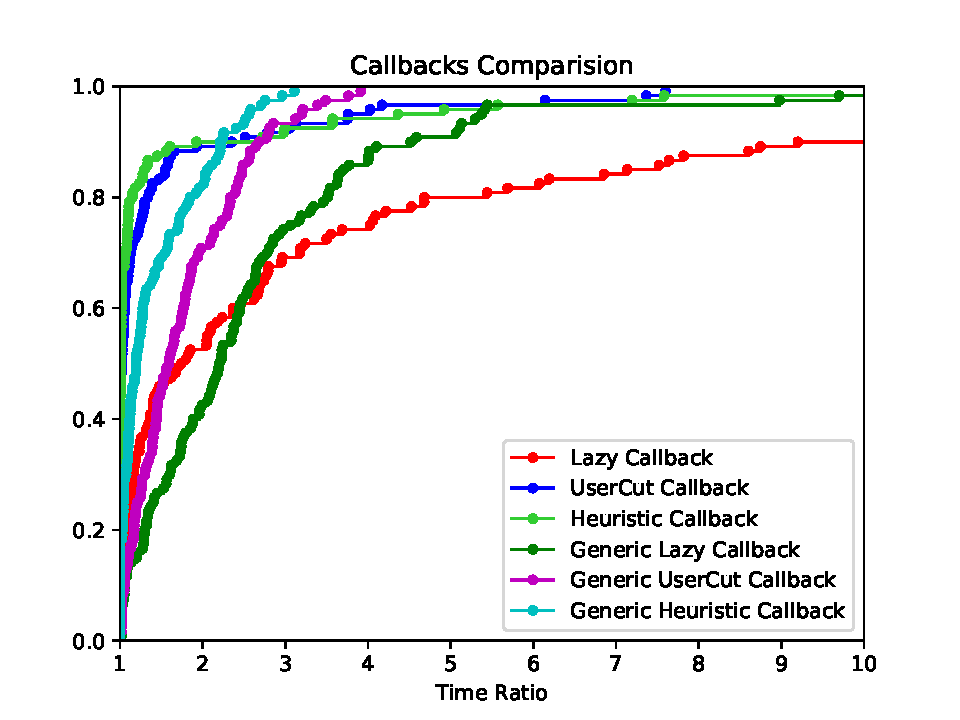
\includegraphics[width=\linewidth]{media/AllCallbacks.pdf}
  \end{subfigure}
  \begin{subfigure}[b]{0.97\linewidth}
  \ContinuedFloat
    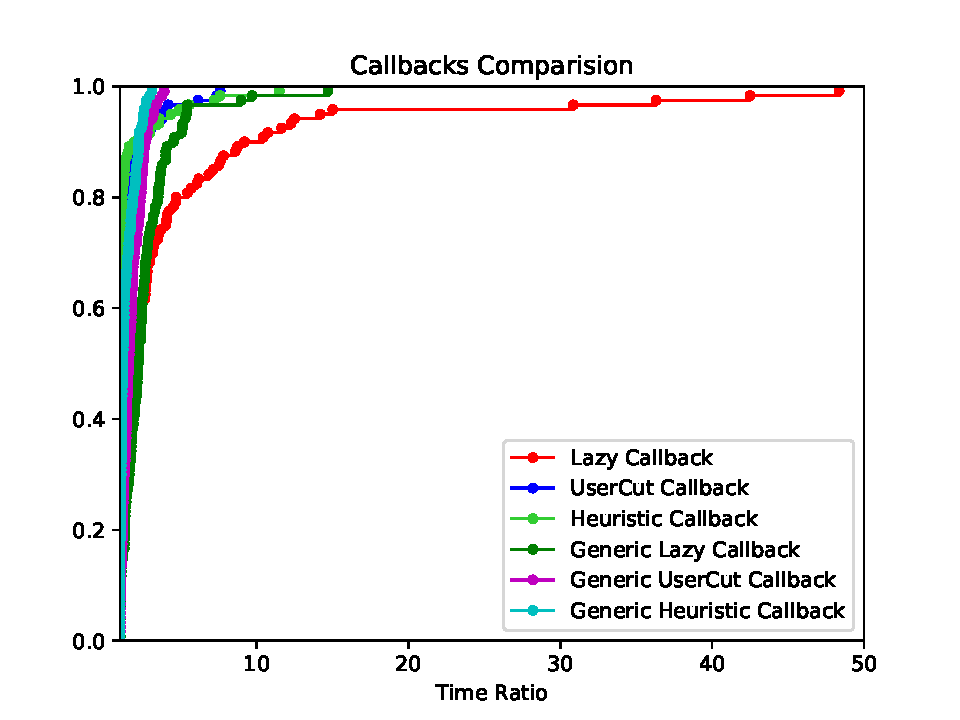
\includegraphics[width=\linewidth]{media/AllCallbacks1.pdf}
  \end{subfigure}
  \caption{On top: detailed view of the performance profile of all Callbacks. \\On the bottom: full view of the performance profile of all Callbacks.}
      \label{fig:allcall}
\end{figure}

\begin{figure}[h!]
  \centering
  \begin{subfigure}[b]{0.97\linewidth}
    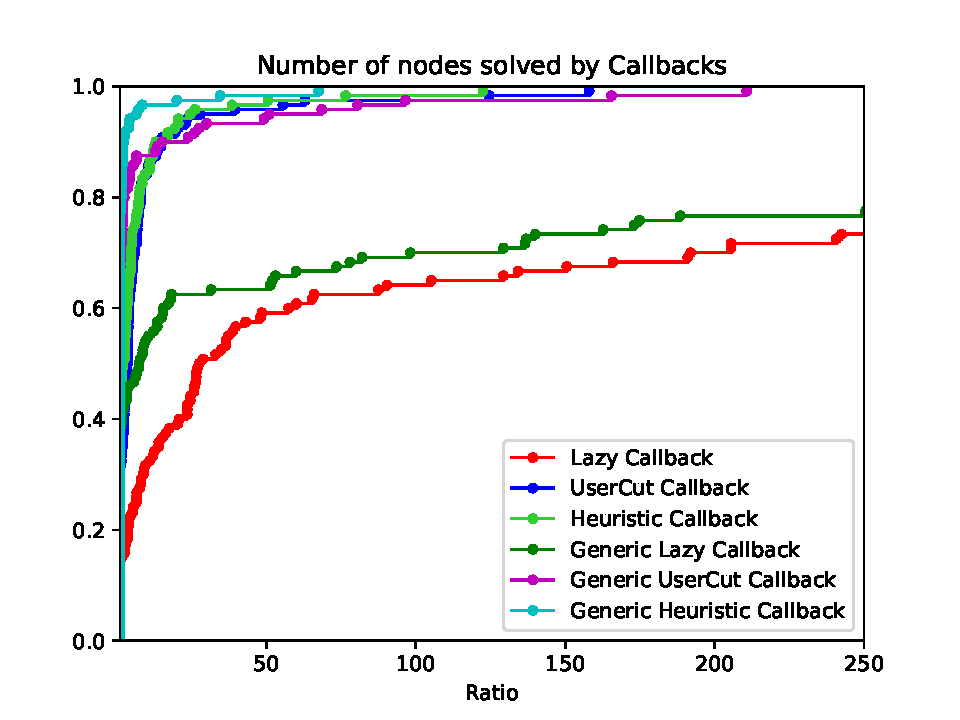
\includegraphics[width=\linewidth]{media/NodesAll.pdf}
  \end{subfigure}
  \begin{subfigure}[b]{0.97\linewidth}
  \ContinuedFloat
    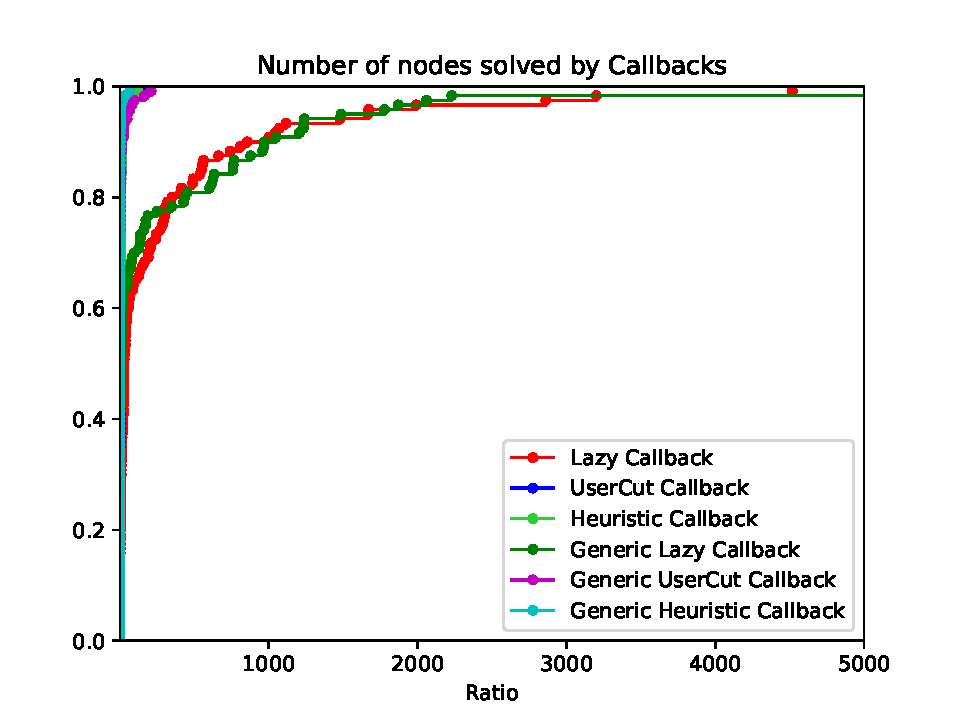
\includegraphics[width=\linewidth]{media/NodesAll1.pdf}
  \end{subfigure}
  \caption{On top: detailed view of the performance profile of all Callbacks regarding the number of solved nodes. On the bottom: full view of the performance profile of all Callbacks.}
       \label{fig:allcallnodes}
\end{figure}

\begin{figure}[h!]
  \centering
  \begin{subfigure}[b]{0.97\linewidth}
    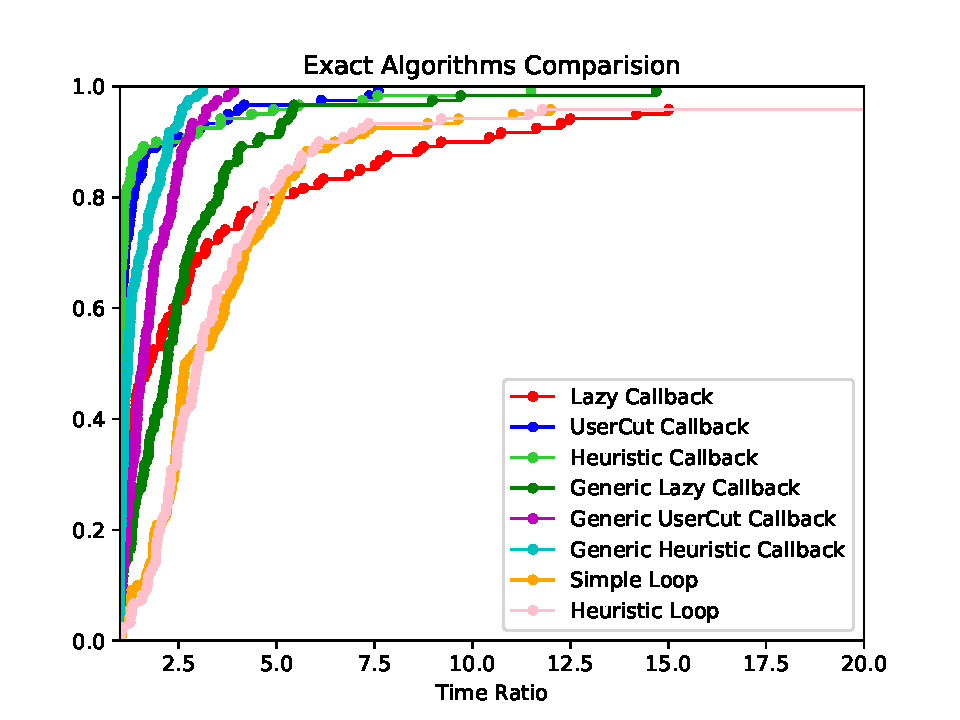
\includegraphics[width=\linewidth]{media/Exact.pdf}
  \end{subfigure}
  \begin{subfigure}[b]{0.97\linewidth}
  \ContinuedFloat
    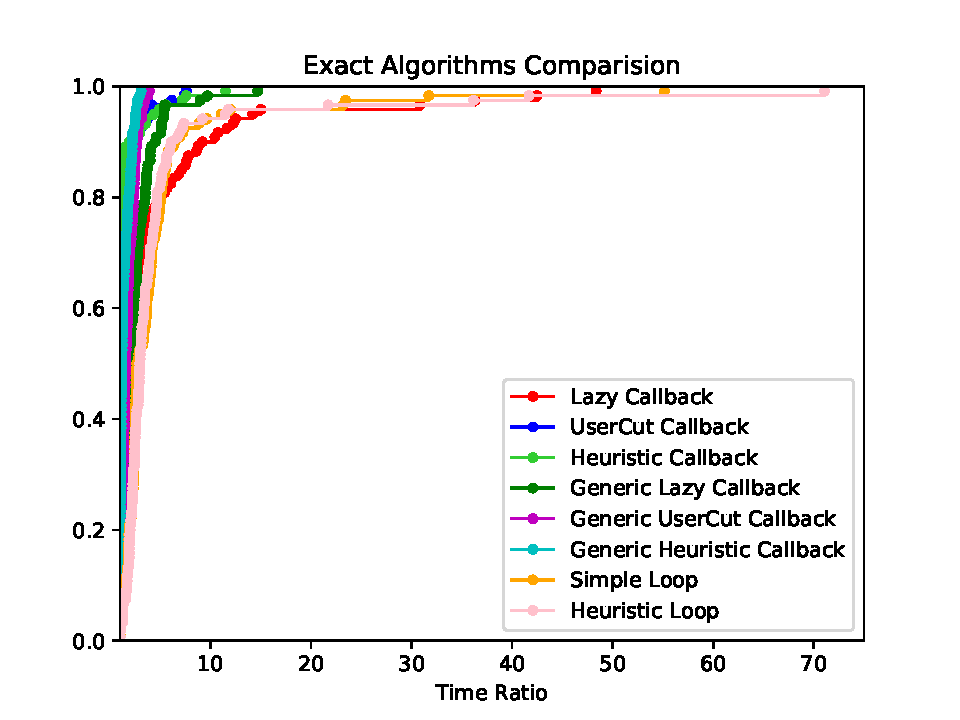
\includegraphics[width=\linewidth]{media/Exact1.pdf}
  \end{subfigure}
  \caption{On top: detailed view of the performance profile of Exact Algorithms. \\On the bottom: full view of the performance profile of Exact Algorithms.}
      \label{fig:exact}
\end{figure}

